\documentclass[10pt]{article}
\usepackage[top=2cm,bottom=2cm,left=2cm,right=2cm]{geometry}
\usepackage[dvipsnames,svgnames,x11names]{xcolor}
\usepackage{multicol}
\usepackage{graphicx}
\usepackage{amsmath,amssymb,amsfonts}
\usepackage{booktabs}
\usepackage{colortbl}
\usepackage{multirow}
\usepackage{tcolorbox}
\usepackage{enumitem}
\usepackage{titlesec}
\usepackage{float}
\usepackage{hyperref}
\usepackage{tabularx}
\setlength{\parindent}{0pt}
\setlength{\parskip}{6pt}

\begin{document}

\begin{center}
{\LARGE\bfseries $\mathbf{T}^{2}$-RAGBench: Text-and-Table Benchmark for Evaluating Retrieval-Augmented Generation}\\[6pt]
Jan Strich$^{1}$, Enes Kutay Isgorur$^{2}$, Maximilian Trescher$^{2}$, Chris Biemann$^{1}$, Martin Semmann$^{1}$\\[4pt]
$^{1}$University of Hamburg, Germany \quad $^{2}$dida Datenschmiede GmbH\\[4pt]
\textit{Correspondence:} \href{mailto:t2ragbench@gmail.com}{t2ragbench@gmail.com}
\end{center}

\section*{Abstract}
Since many real-world documents combine textual and tabular data, robust Retrieval Augmented Generation (RAG) systems are essential for effectively accessing and analyzing such content to support complex reasoning tasks. Therefore, this paper introduces $\mathbf{T}^2$-RAGBench, a benchmark comprising 23,088 question-context-answer triples, designed to evaluate RAG methods on real-world text-and-table data. Unlike typical QA datasets that operate under \textit{Oracle Context} settings, $\mathbf{T}^2$-RAGBench challenges models to first retrieve the correct context before conducting numerical reasoning. Existing QA datasets containing text-and-table data typically contain context-dependent questions, which may yield multiple correct answers depending on the provided context. To address this, we transform SOTA datasets into a context-independent format, validated by experts as 91.3\% context-independent questions, enabling reliable RAG evaluation. Our comprehensive evaluation identifies \textit{Hybrid BM25}, a technique that combines dense and sparse vectors, as the most effective approach for text-and-table data. However, results demonstrate that $\mathbf{T}^2$-RAGBench remains challenging even for SOTA LLMs and RAG methods. Further ablation studies examine the impact of embedding models and corpus size on retrieval performance. $\mathbf{T}^2$-RAGBench provides a realistic and rigorous benchmark for existing RAG methods on text-and-table data. Code and dataset are available online$^1$.

\section{Introduction}
Documents containing a mixture of text and tables are widely utilized in various fields, such as financial reporting (Baviskar et al., 2021), scientific research (Pramanick et al., 2024), and organizational documentation (Rebman Jr et al., 2023).

Recent advancements in Large Language Models (LLMs) have demonstrated solid SOTA performance answering numerical and free-form question-answering (QA) tasks when appropriate documents are provided (Nan et al., 2021; Chen et al., 2021, 2022; Zhu et al., 2021, 2022). Despite increasing context window sizes for LLMs, using the entire corpus remains impractical due to computational constraints and programmatic latency (Wang et al., 2024b; Li et al., 2024). Therefore, retrieving relevant documents is essential in real-world applications to answer questions correctly.

Retrieval-Augmented Generation (RAG) (Lewis et al., 2020) has emerged as a promising solution for single-hop QA on numerical tasks, providing appropriate context and has led to an explosion of methods in this area (Gao et al., 2023b; Nikishina et al., 2025). While most RAG methods are effective at retrieving semantically similar text, embedding tabular data remains challenging due to its structural complexity and the predominance of numerical values, which lack semantic context (Khattab et al., 2022).

\begin{figure}[H]
    \centering
    \begin{minipage}{0.45\textwidth}
        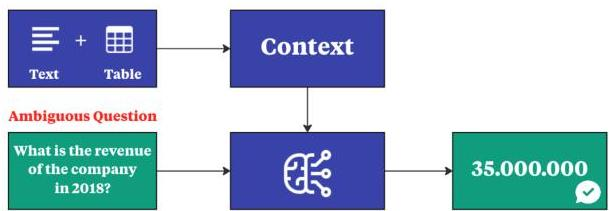
\includegraphics[width=\linewidth]{figures/part1_img-0.jpeg}\\
        \centering a) Oracle-Context Setting
    \end{minipage}\hfill
    \begin{minipage}{0.45\textwidth}
        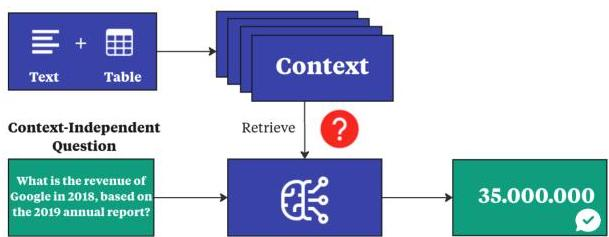
\includegraphics[width=\linewidth]{figures/part1_img-1.jpeg}\\
        \centering b) Unknown-Context Setting
    \end{minipage}
    \\[-4pt]
    \caption{Overview of current SOTA approaches and dataset example. a) Most benchmarks test models in an \textit{Oracle Context} setting, (Chen et al., 2021, 2022). Our task (b) targets the unknown-context setting, requiring retrieval from mixed text-tables before answering.}
\end{figure}

In addition, RAG methods are typically trained and evaluated on text-only datasets (Jiang et al., 2023; Lan et al., 2023; Wang et al., 2024b), Wikipedia-derived QA benchmarks (Pasupat and Liang, 2015; Yang et al., 2018) heavily used during LLM pre-training (Grattafiori et al., 2024), or narrow domain-specific datasets (Sarthi et al., 2024; Yan et al., 2024), making it difficult to estimate the performance on text-and-table data. Moreover, as illustrated in Figure 1, existing datasets with text-and-table data operate exclusively under the oracle context setting, where questions are tightly coupled with the given context. These questions are inherently ambiguous and may yield multiple correct answers depending on the context, we refer to them as \textit{context-dependent}. In contrast, \textit{context-independent} questions have a single correct answer without having access to the context, which is essential for evaluating RAG methods, as they require identifying one ground truth document containing the answer. To our knowledge, no text-and-table dataset meets this requirement.

To fill this gap, we present the Text-Table Retrieval-Augmented Generation Benchmark ($T^{2}$-RAGBench), a benchmark designed to evaluate existing RAG methods on text-table retrieval and numerical reasoning tasks. Our benchmark comprises three subsets extracted from existing datasets, totaling 23,088 question-context-answer (QCA) triples and 7,318 real-world financial documents. Each triplet includes a reformulated, context-independent question, a verified answer, and the associated context containing all information to answer the question.

Our contributions are as follows:
\begin{itemize}
    \item We introduce $T^{2}$-RAGBench, a benchmark containing 23,088 QCA triples from financial reports designed to evaluate RAG methods on text-and-table and numerical reasoning.
    \item We systematically evaluate popular RAG methods on $T^{2}$-RAGBench, demonstrating that it remains a challenging and relevant benchmark for current methods.
    \item We compare SOTA closed and open-source embedding models and analyze the effect of corpus size on promising RAG methods.
\end{itemize}

\section{Related Work}
\subsection*{Text-and-Table QA Datasets}
Table~\ref{tab:datasets} gives an overview of existing Q\&A datasets containing text and/or tables. While datasets in common knowledge (Joshi et al., 2017; Chen et al., 2020; Nan et al., 2021), scientific documents (Pramanick et al., 2024; Dasigi et al., 2021), or medicine (Fan et al., 2025) focusing exclusively on tables (Katsis et al., 2022), combining text with tables becomes essential for effectively parsing whole PDF documents. Another challenge is data contamination, as common knowledge and scientific datasets often rely on Wikipedia or open-access papers, which are heavily used during LLM pretraining (Grattafiori et al., 2024). This makes it difficult to separate retriever and generator performance in RAG evaluation.

In other domains, such as finance, VQAonBD (Raja et al., 2023) focuses also only on tables, but FinQA (Chen et al., 2021), ConvFinQA (Chen et al., 2022), and TAT-DQA (Zhu et al., 2022) incorporate both text-and-tabular data from financial reports. Nonetheless, all financial datasets contain mainly context-dependent questions.

Moreover, several datasets are not publicly available, such as FinDER (Choi et al., 2025) and BioTABQA (Luo et al., 2022), or represent tables as images rather than structured text in markdown format (Tito et al., 2021; Pramanick et al., 2024). Other datasets are cross-domain, such as TableBench (Wu et al., 2025), which provides multi-domain table QA for oracle context evaluation, while the UDA benchmark (Hui et al., 2024) aggregates multiple datasets. However, both remain limited by context-dependent questions. $T^{2}$-RAGBench closes this gap by providing a benchmark that focuses on text-and table-data, has no data contamination, and contains only context-independent questions.

\subsection*{RAG on Text-and-Table}
RAG shows promise on text (Lewis et al., 2020), but text-and-table evaluation is limited. THoRR (Kim et al., 2024) simplifies tables via header-based retrieval, complementing ERATTA (Roychowdhury et al., 2024), which uses modular prompts and SQL for enterprise data. FinTextQA (Chen et al., 2024) evaluates full RAG pipelines. FinTMMBench (Zhu et al., 2025) adds multi-modal and temporal RAG via dense/graph retrieval. Robust RAG (Joshi et al., 2024) links text, tables, visuals via image-based VLLMs, though less flexible than text methods. Despite progress, most works (Asai et al., 2024; Gao et al., 2023a,b) test only a few RAG baselines, limiting generalizability.

\begin{table*}[t]
\centering
\caption{Summary and comparison of Q\&A datasets. Visual Independence: The contexts are presented as text and are not only images. Context-Independent: Without a context, questions still only have one unambiguous answer.}
\label{tab:datasets}
\begin{tabular}{l l c c c c c r}
\toprule
Dataset & Domain & Text & Table & Visual Independence & Context-Independent & Available & QA Pairs \\
\midrule
TriviaQA (Joshi et al., 2017) & Wikipedia & $\checkmark$ & $\times$ & $\checkmark$ & $\checkmark$ & $\checkmark$ & 650K \\
HybridQA (Chen et al., 2020) & Wikipedia & $\times$ & $\checkmark$ & $\checkmark$ & $\checkmark$ & $\checkmark$ & 70K \\
FeTaQA (Nan et al., 2021) & Wikipedia & $\times$ & $\checkmark$ & $\checkmark$ & $\checkmark$ & $\checkmark$ & 10K \\
Qasper (Dasigi et al., 2021) & NLP Papers & $\times$ & $\checkmark$ & $\checkmark$ & $\times$ & $\checkmark$ & 5K \\
SPIQA (Pramanick et al., 2024) & NLP Papers & $\times$ & $\checkmark$ & $\times$ & $\times$ & $\checkmark$ & 270K \\
FinQA (Chen et al., 2021) & Finance & $\checkmark$ & $\checkmark$ & $\checkmark$ & $\times$ & $\checkmark$ & 8K \\
ConvFinQA (Chen et al., 2022) & Finance & $\checkmark$ & $\checkmark$ & $\checkmark$ & $\times$ & $\checkmark$ & 14K \\
TAT-DQA (Zhu et al., 2022) & Finance & $\checkmark$ & $\checkmark$ & $\checkmark$ & $\times$ & $\checkmark$ & 16K \\
VQAonBD (Raja et al., 2023) & Finance & $\times$ & $\checkmark$ & $\times$ & $\times$ & $\checkmark$ & 1,531K \\
FinDER (Choi et al., 2025) & Finance & $\checkmark$ & $\checkmark$ & $\checkmark$ & $\checkmark$ & $\times$ & 50K \\
DocVQA (Tito et al., 2021) & Multiple & $\times$ & $\checkmark$ & $\times$ & $\times$ & $\checkmark$ & 50K \\
TableBench (Wu et al., 2025) & Multiple & $\checkmark$ & $\checkmark$ & $\times$ & $\times$ & $\checkmark$ & $\sim$1K \\
UDA (Hui et al., 2024) & Multiple & $\checkmark$ & $\checkmark$ & $\checkmark$ & $\times$ & $\checkmark$ & 30K \\
\textbf{$T^{2}$-RAGBench (Ours)} & Finance & $\checkmark$ & $\checkmark$ & $\checkmark$ & $\checkmark$ & $\checkmark$ & 23K \\
\bottomrule
\end{tabular}
\end{table*}

\section{Task Definition}
To clarify the task addressed by our benchmark, we define the following problem to be solved.

\textbf{Problem Formulation.} The benchmark evaluates both the retrieval function $f$ and the reasoning model $M$ to optimize answer accuracy and efficiency in the unknown-context text-and-table QA setting. We denote the user's question by $Q$ and the corresponding ground truth answer by $A$. The evidence comes from two modalities: a segment of text content and a structured table, which we consider together as a single context entity denoted by $C$. Thus, our entire context corpus is defined as $\mathcal{C} = \{C_i\}$. The task is divided into two stages:

\textbf{Retrieval:} A function
\begin{equation}
f: \mathcal{C} \times Q \mapsto \left[ C_{k \mid k = 1}^{*} \right]^{n}
\end{equation}
selects the top-$n$ most relevant context entities from the corpus $\mathcal{C}$ for a given question $Q$.

\textbf{Answer Extraction:} A language model
\begin{equation}
M: \left(\left[ C_{k \mid k = 1}^{*} \right]^{n}, Q\right) \mapsto A^{*}
\end{equation}
generates an answer $A^{*}$ by reasoning over the retrieved text and tables.

\textbf{Number Match:} Numerical reasoning is evaluated using a new metric. It allows for minor deviations and unit scale shifts. Let $A^{*}$ and $A$ be the predicted and ground truth answers, and denote their absolute values as $a^{*} = |A^{*}|$ and $a = |A|$. Given a tolerance threshold $\varepsilon > 0$, the prediction is considered correct if either $a^{*} < \varepsilon$ and $a < \varepsilon$, or $|q - 1| < \varepsilon$ where
\begin{equation}
q = \frac{a^{*}}{a} \cdot 10^{-\mathrm{round}(\log_{10}(a^{*}/a))}.
\end{equation}
Here, round denotes rounding to the nearest integer. This metric ensures robustness to rounding errors and magnitude scaling.

\textbf{Retrieval Metrics.} Let
\begin{equation}
\mathcal{D} = \left\{\left(Q_{i}, A_{i}, C_{i}\right) \right\}_{i = 1}^{N}
\end{equation}
represent our dataset, where each tuple $(Q_{i}, A_{i}, C_{i})$ consists of a question $Q_{i}$, its unique ground-truth answer $A_{i}$, and the corresponding unique ground-truth context $C_{i}$. Define the retrieval output:
\begin{equation}
R_{i} = f(\mathcal{C}, Q_{i}) = \left[ C_{i, 1}^{*}, C_{i, 2}^{*}, \dots, C_{i, n}^{*} \right].
\end{equation}
The true rank is given by
\begin{equation}
r_{i} = \min \left\{k \mid C_{i, k}^{*} = C_{i} \right\}.
\end{equation}
We consider the Mean Reciprocal Rank at $k$ (MRR@k), which focuses on the relevance of the top $k$ retrieved contexts. It is defined as
\begin{equation}
\operatorname{MRR}@k = \frac{1}{N} \sum_{i = 1}^{N} \frac{1}{r_{i}} \cdot \mathbb{I}(r_{i} \leq k),
\end{equation}
where $\mathbb{I}(\cdot)$ is the indicator function, valued at 1 if the condition is met (i.e., $r_i \leq k$), and 0 otherwise.

\begin{table*}[t]
\centering
\begin{tabular}{|l|l|l|r|r|r|r|r|r|r|}
\hline
Subset & Domain & PDF Source & \multicolumn{3}{c|}{\#Documents} & \multicolumn{2}{c|}{\#QA Pairs} & \multicolumn{2}{c|}{Avg. Question Tokens} \\
\cline{4-10}
 & & & Original & Extracted & Avg. Token & Original & Generated & Original & Generated \\
\hline
FinQA & Finance & FinTabNet & 2,789 & 2,789 & 950.4 & 8,281 & 8,281 & 21.1 & 39.2 \\
ConvFinQA & Finance & FinTabNet & 2,066 & 1,806 & 890.9 & 14,115 & 3,458 & 17.8 & 30.9 \\
TAT-DQA & Finance & TAT-DQA & 2,758 & 2,723 & 915.3 & 16,558 & 11,349 & 17.8 & 31.7 \\
\hline
Total & Finance & Multiple & 7,613 & 7,318 & 924.2 & 38,954 & 23,088 & 19.0 & 34.3 \\
\hline
\end{tabular}
\caption{Comparison of original and generated QA pairs, documents, and average question and context lengths across $\mathrm{T}^2$-RAGBench subsets. FinQA (Chen et al., 2021) and ConvFinQA (Chen et al., 2022) use FinTabNet (Zheng et al., 2021) as their PDF source, while TAT-DQA (Zhu et al., 2022) uses its own dataset. Avg. token count based on Llama 3.3 tokenizer.}
\end{table*}

\section{$T^2$-RAGBench}
To construct our benchmark for text-table data suitable for RAG evaluation, we first surveyed existing datasets, as summarized in Table 1. As none fully met our criteria, we selected FinQA (Chen et al., 2021), ConvFinQA (Chen et al., 2022), and TAT-DQA (Zhu et al., 2022) and restructured them to context-independent questions.

A question is considered context-independent if it has exactly one correct answer, even without access to $\mathcal{C}$. For all selected datasets, we applied custom preprocessing steps and reformulated questions using Llama 3.3-70B\footnote{\url{https://huggingface.co/kosbu/Llama-3.3-70B-Instruct-AWQ}} to ensure context-independence.

Each benchmark sample is a triple $(Q, A, C)$, where $Q$ is a question, $A$ the answer, and $C$ the context composed of both text and table. Since all triples originate from Oracle Context settings, we assume that all required information to answer $Q$ is fully contained within $C$, and only within $C$. Table 2 provides a detailed breakdown of the three subsets of $\mathrm{T}^2$-RAGBench. While FinQA and ConvFinQA are based on FinTabNet, TAT-DQA is based on its own financial documents. The subsets consist of 1,806 to 2,789 documents, with each containing between 3,458 and 11,349 QA pairs. We included samples for each subset in Appendix A.

\subsection{Data Preparation}
All subsets required tailored preprocessing to align with the requirements of our benchmark. FinQA is a numerical QA dataset based on financial reports from FinTabNet. We used it with company metadata and standardized all answer formats. ConvFinQA extends FinQA by adding multi-turn questions. We filtered only to include first-turn questions and normalized the answers for consistency. TAT-DQA is an independent dataset with diverse answer types. We filtered it to keep only numerical questions and normalized answer formats. Full details can be found in Appendix B.

\subsection{Data Creation}
Following the preprocessing, the context-independent questions were generated. First, the questions were reformulated using an LLM. Subsequently, both quantitative and qualitative analyses were performed to verify that (1) the data quality remained consistent with the original, and (2) the reformulation process produced genuinely context-independent questions.

\textbf{Question Reformulation.} To generate context-independent questions, the original questions were reformulated, but the answers remained unchanged to preserve human-annotated quality. For each of the 23,088 samples, a new question was generated using Llama 3.3-70B with temperature $=0.7$. The generation process was conducted by incorporating meta-information, such as company name, sector, and report year, which were not included in the original document. The exact prompting template is detailed in Appendix C.

\textbf{Quantitative Analysis.} To verify that the rephrased questions remain consistent with the original answer, we conducted a quantitative comparison of the original and reformulated questions across all subsets using Llama 3.3-70B and Oracle Context, as presented in Figure~\ref{fig:number_match}.

Since the context is given, only Number Match was used to evaluate the QA pairs. The accuracy between original and generated questions shows minimal deviation, with maximal differences of $2\%$ per subset and in average $<0.05\%$. The ability of the LLM to answer the reformulated questions indicates that they retain the essential information required for numerical reasoning.

\begin{figure*}[t]
    \centering
    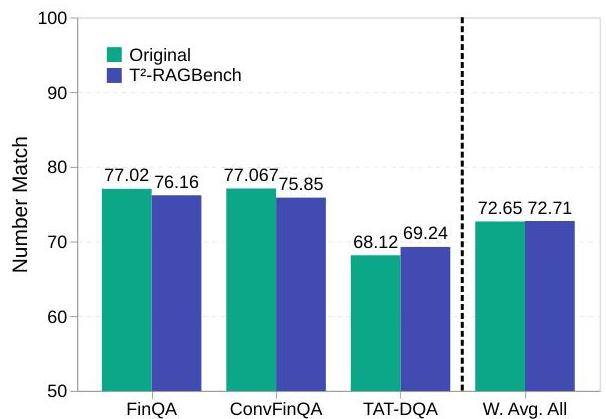
\includegraphics[width=0.8\textwidth]{figures/part1_img-2.jpeg}
    \caption{Number Match comparison per subset and weighted average all between original and reformulated questions from our new benchmark.}
    \label{fig:number_match}
\end{figure*}

\textbf{Human Validation.} To further investigate whether the questions are now context-independent after reformulation, we conducted a human evaluation after the quantitative analysis. Therefore, a random sample of 100 original and generated QA pairs per subset was manually labeled via a custom annotation tool (Appendix D). Each of the four financial experts annotated 200 samples from two different subsets, assessing whether the original questions were context-independent or context-dependent. The analysis reveals that only $11.8\%$ of questions in the original dataset were context-independent, compared to $93\%$ in the reformulated version (see Figure~\ref{fig:context_independence}). This ensures that nearly all of the newly created QCA triples are suitable for RAG evaluation. Cohen's Kappa was calculated to assess inter-annotator agreement, yielding an overall value of 0.87, indicating almost perfect agreement. Notably, only $1/3$ of the uncertain cases involved reformulated questions, suggesting that most ambiguity stemmed from original question formulations. For better transparency, we include representative disagreement examples in Appendix E and in our repository\footnote{\url{https://huggingface.co/datasets/T2-RAGBench}}.

\subsection{Data Statistics}
Table 2 presents an overview of the dataset. It comprises 7,318 real-world documents with an average length of 924.2 tokens. In total, $\mathrm{T}^2$-RAGBench consists of 23,088 QCA triples extracted from roughly 40k questions. Questions increased by $\sim 15$ tokens with added semantic details (e.g., company names, years), making them context-independent and suitable for RAG evaluation. All other parameters (Metadata, IDs, etc.) of the dataset remained the same.

\begin{figure*}[t]
    \centering
    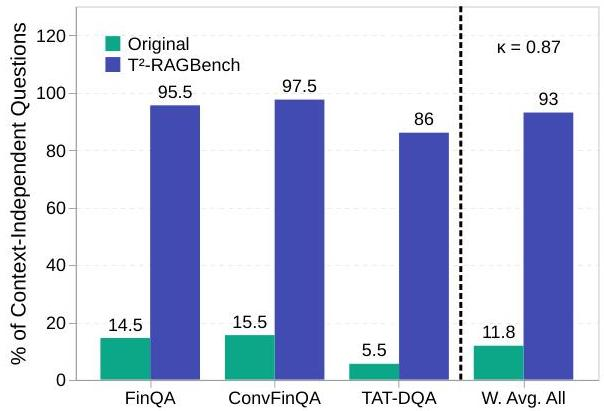
\includegraphics[width=0.8\textwidth]{figures/part1_img-3.jpeg}
    \caption{Percentage of context-independent questions (100 per subset, weighted avg overall). $\kappa$ indicates inter-annotator agreement.}
    \label{fig:context_independence}
\end{figure*}

\section{Experiments}
To evaluate the suitability of our benchmark for RAG methods, we report results across all subsets using various models and RAG approaches. This section describes the setup (Section~5.1), compares methods (Section~5.2), defines metrics (Section~5.3), and presents the main results (Section~5.4), revealing a large gap between oracle and current RAG performance. We then analyze this gap via two ablations (Section~5.5) and a manual error analysis (Section~5.6).

\subsection{Experimental Setup}
For the evaluation of the benchmark, each subset was evaluated independently. First, all contexts were transformed into markdown format and uniquely stored into a Chroma (Chroma Team, 2025) vector db using the embeddings created with the multilingual e5-large instruct model (Wang et al., 2024a), having an embedding size of 1024. That was done for all RAG methods except for Summarization and SumContext, where the summarized context was embedded. A retrieval query was used to retrieve from the embedding model (See Appendix F). The Top-3 documents were selected and passed to the generator in the main evaluation. As generators, we employed quantized LLaMA 3.3-70B, a decoder-only transformer, and QwQ-32B\footnote{\url{https://huggingface.co/Qwen/QwQ-32B-AWQ}}, to evaluate performance across multiple model architectures on two NVIDIA H100. Due to resource limitations, we utilize quantized models, which exhibit negligible performance loss (Jin et al., 2024). The prompt template is provided in Appendix G.

\subsection{RAG Methods}
The following section briefly describes all evaluated RAG methods to show the SOTA performance on $T^{2}$-RAGBench, categorized by the retrieval complexity and augmentation strategy.

\paragraph{Pretrained-Only and Oracle Context.} In the \textit{Pretrained-Only} setup, no retriever is employed, and models must answer questions solely based on their pretraining knowledge. Conversely, the \textit{Oracle Context} setting assumes that the relevant context is directly passed to the generator.

\paragraph{Basic RAG Methods.} This category includes approaches that retrieve documents using standard embedding-based methods. The \textit{Base RAG} implementation follows the original RAG approach (Lewis et al., 2020), where only the question is embedded to retrieve the top-$k$ documents, which are then passed unchanged to the generator. \textit{Hybrid BM25} (Gao et al., 2021) combines sparse lexical retrieval using BM25 with dense vector retrieval, leveraging both methods to improve recall and relevance. Additionally, the \textit{Reranker} method (Glass et al., 2022) applies a cross-encoder model\footnote{huggingface.co/cross-encoder/ms-marco-MiniLM-L6-v2} after initial retrieval to reorder documents based on their relevance in a shared embedding space.

\paragraph{Advanced RAG Methods.} This category consists of methods that modify the query, transform retrieved contexts, or employ iterative retrieval strategies. The \textit{HyDE} method (Gao et al., 2023a) generates hypothetical answers for each question, using them as refined queries to retrieve more relevant documents (For prompt see Appendix H). \textit{Summarization} reduces noise by summarizing each retrieved context using an LLM, focusing on essential information. \textit{SumContext} applies the similar summarization step but retains the original full documents for generation, aiming to reduce distractions while preserving content fidelity (See Appendix I).

\subsection{Evaluation Metrics}
We use Number Match and MRR@$k$ as our main metrics as defined in Section 3, but also report Recall@$k$ for better comparability and transparency. Number Match evaluates if a numerical numerical prediction closely matches the gold numerical answer. It compares predicted and ground truth values using relative tolerance ($\epsilon=1\mathrm{e}{-2}$), accounting for scale invariance. Non-numeric predictions or mismatches are considered incorrect. For MRR and Recall, we choose $k=3$, which measures whether the first relevant document appears in the top-3 retrieved results, rewarding higher ranks for MRR. We limit evaluation to 3 documents, as the average length is 924.2 tokens. Increasing the number of documents increases input size, slows inference, and hinders LLM performance, making it impractical (Li et al., 2024).

\subsection{Main Results}
This section discusses our main results presented in Table 3 for all three evaluation subcategories.

\paragraph{Pretrained-Only and Oracle Context.} The results from the \textit{Pretrained-Only} setting show that across all subsets, the questions cannot be answered directly from the models’ pretraining data. This highlights the importance of RAG and the need for a dedicated benchmark. While reformulated questions may resemble seen content, especially since most S\&P 500 reports predate 2023, this applies to both foundation and reasoning models. In contrast, the \textit{Oracle Context} setting shows consistently high performance on Number Match across all subsets and both models, highlighting both the strong numerical reasoning abilities of the models and the feasibility of the task for modern LLMs in this setting. Notably, there is no significant performance difference between Llama and QwQ ($<0.3\%$).

\paragraph{Base RAG Methods.} For base RAG methods, the benchmark shows that all SOTA models still struggle to match the performance achieved in \textit{Oracle Context}. Nevertheless, this benchmark offers the possibility to compare the different methods precisely. For \textit{Base-RAG}, MRR@3 and R@3 averaging below 40\%, meaning relevant documents are often missing in the top-3, which leads to a significant drop in Number Match. This effect is particularly evident in TAT-DQA, where, despite having a similar number of documents as FinQA, relevant information is harder to retrieve for all tested methods. \textit{Hybrid BM25} consistently outperforms base RAG in Number Match, MRR@3, and R@3 on average. Interestingly, the \textit{Reranker} performs worse than Base and Hybrid BM25 RAG methods, suggesting that the reranking model struggles with text-and-table data.

\paragraph{Advanced RAG Methods.} One way to improve the performance of RAG methods is to improve the linking of the query with the context. However, \textit{HyDE} shows even a drop in performance in

\begin{table*}[h!]
\centering
\scriptsize
\begin{tabular}{ll|ccc|ccc|ccc|ccc}
\toprule
Model & RAG Method & \multicolumn{3}{c|}{FinQA} & \multicolumn{3}{c|}{ConvFinQA} & \multicolumn{3}{c|}{TAT-DQA} & \multicolumn{3}{c}{W. Avg Total} \\
& & NM & MRR@3 & R@3 & NM & MRR@3 & R@3 & NM & MRR@3 & R@3 & NM & MRR@3 & R@3 \\
\midrule
\multirow{8}{*}{\begin{tabular}[c]{@{}l@{}}Llama 3.3-70B \\ + Multilingual \\ E5-Large \\ Instruct\end{tabular}} & + Pretrained-Only & 7.9 & - & - & 2.8 & - & - & 3.7 & - & - & 5.1 & - & - \\
& + Oracle Context & 76.2 & 100 & 100 & 75.8 & 100 & 100 & 69.2 & 100 & 100 & 72.7 & 100 & - \\
& + Base-RAG & 39.5 & 38.7 & 49.7 & 47.4 & 42.2 & 53.8 & 29.6 & 25.2 & 28.4 & 35.8 & 32.6 & 39.8 \\
& + Hybrid BM25 & 41.7 & 40.0 & 53.0 & 50.3 & 43.5 & 57.2 & 37.4 & 29.2 & 44.4 & 40.9 & 35.2 & 49.4 \\
& + Reranker & 32.4 & 29.0 & 36.2 & 37.3 & 32.3 & 40.5 & 27.0 & 22.8 & 28.4 & 30.5 & 26.4 & 33.0 \\
& + HyDE & 38.4 & 35.4 & 45.7 & 44.8 & 39.8 & 50.9 & 26.7 & 20.8 & 26.7 & 33.6 & 28.9 & 37.1 \\
& + Summarization & 27.3 & 47.3 & 59.5 & 35.2 & 52.1 & 63.8 & 14.6 & 24.7 & 31.5 & 22.2 & 36.9 & 46.4 \\
& + SumContext & 47.2 & 47.3 & 59.4 & 55.5 & 52.1 & 63.8 & 29.1 & 24.8 & 31.4 & 39.5 & 37.0 & 46.3 \\
\midrule
\multirow{8}{*}{\begin{tabular}[c]{@{}l@{}}QwQ-32B \\ + Multilingual \\ E5-Large \\ Instruct\end{tabular}} & + Pretrained-Only & 7.5 & - & - & 2.4 & - & - & 4.4 & - & - & 5.2 & - & - \\
& + Oracle Context & 72.4 & 100 & - & 85.4 & 100 & - & 71.1 & 100 & - & 73.7 & 100 & - \\
& + Base-RAG & 39.6 & 38.7 & 49.7 & 48.7 & 42.4 & 53.8 & 27.9 & 25.2 & 28.4 & 35.2 & 32.6 & 39.8 \\
& + Hybrid BM25 & 41.8 & 39.8 & 53.0 & 51.6 & 43.6 & 57.2 & 37.2 & 29.3 & 44.4 & 41.0 & 35.2 & 49.4 \\
& + Reranker & 30.8 & 29.0 & 36.2 & 37.5 & 32.7 & 40.5 & 25.6 & 22.9 & 28.4 & 29.2 & 26.6 & 33.0 \\
& + HyDE & 36.8 & 35.4 & 45.7 & 45.7 & 39.9 & 50.9 & 24.7 & 20.7 & 26.7 & 32.2 & 28.8 & 37.1 \\
& + Summarization & 26.9 & 47.2 & 59.5 & 35.6 & 52.2 & 63.8 & 13.9 & 24.7 & 31.5 & 21.8 & 36.9 & 46.4 \\
& + SumContext & 45.6 & 47.3 & 59.4 & 56.9 & 52.2 & 63.8 & 27.3 & 24.7 & 31.4 & 38.3 & 36.9 & 46.3 \\
\bottomrule
\end{tabular}
\caption{Overall performance (Number Match (NM), MRR@3, and R@3) of both models on $\mathrm{T}^2$-RAGBench. Number Match represents the percentage of correctly answered questions based on their numerical representation. R@3 and MRR@3 evaluate retrieval effectiveness. Cells in Bold indicate the highest value over all RAG methods, and underlined indicate the best value across RAG method categories.}
\end{table*}

MRR@3 and R@3 across all subsets in comparison to the \textit{Base-RAG}. This may be due to the models' difficulty in generating well-structured content matching the format of the documents, which often include both text and tables.

The \textit{Summarization} approach performed well on MRR@3 for FinQA and ConvFinQA by condensing relevant information and removing noise. However, it underperforms on TAT-DQA, warranting further investigation. In general, this often led to a drop in NM, as essential information needed to answer the questions was also lost during summarization. \textit{SumContext} retrieves from a summarized context but provides the full original context. This approach improved MRR@3 while maintaining stable NM, achieving an average NM of $37.4\%$ resp. $36.7\%$. Nevertheless, the performance does not improve across all subsets, indicating strong sensitivity to prompts and datasets. Interestingly, MRR@3 is $1.8\%$ higher than \textit{Hybrid BM25}, despite lower R@3, suggesting retrieved documents are ranked higher in Summarization and SumContext.

\subsection*{5.5 Ablation Studies}
\textbf{Embedding Models.} We evaluate various embedding models with the \textit{Base-RAG} approach to assess their impact on retrieval performance. As shown in Table 4, among the open-source models, \textit{Multilingual E5-Instruct} performs best, achieving $29.4\%$ R@1 and 38.6 MRR@5. The closed-source models perform slightly better, with the OpenAI model reaching the highest R@1 of $33.8\%$ and MRR@5 of 43.6. However, none of the models, regardless of model size, achieve satisfactory performance on the challenging text-and-table setting at R@1, indicating that retrieving the correct document remains a core challenge in $\mathrm{T}^2$-RAGBench, because text-and-table documents seem to be challenging for SOTA embedding models.

\begin{table}[H]
\centering
\begin{tabular}{lccc}
\toprule
Embedding Model & R@1 & R@5 & MRR@5 \\
\midrule
Stella-EN-1.5B & 2.2 & 5.2 & 3.3 \\
GTE-Qwen2 1.5B Instruct & 12.5 & 27.6 & 18.0 \\
Multilingual E5-Instruct & 26.4 & 49.7 & 35.1 \\
Gemini: Text-Embedding-004 & 32.3 & 53.6 & 41.7 \\
OpenAI: Text-Embedding-3 Large & 34.6 & 57.4 & 44.7 \\
\bottomrule
\end{tabular}
\caption{Retrieval performance of embedding models on $\mathrm{T}^2$-RAGBench using Base-RAG with $k = 5$ retrieved documents, evaluated on R@1, R@5 and MRR@5. Scores are weighted avg. over all subsets. Model descriptions are in Appendix J.}
\end{table}

\textbf{Number of Documents.} Figure 4 shows how retrieval performance changes with the number of documents for \textit{Base-RAG} and \textit{Summarization}, using 5 random percentage ascending subsets per dataset. Two main findings emerge: (1) MRR@3 drops below $50\%$ with 3K documents, meaning the correct document appears in the top 3 only half the time; (2) Summarization improves results for FinQA and ConvFinQA, performs similarly on TAT-DQA, where summarizing tabular content is more challenging.

\begin{figure}[H]
    \centering
    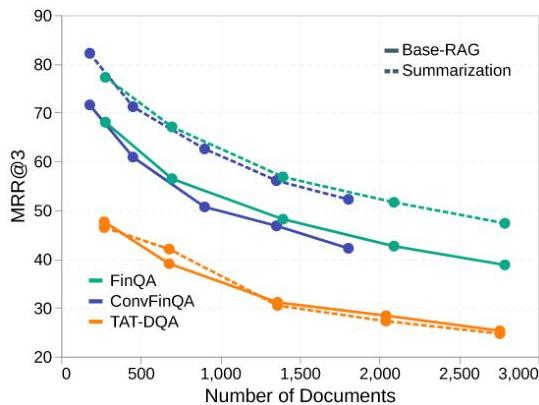
\includegraphics[width=0.8\linewidth]{figures/part2_img-0.jpeg}
    \caption{MRR@3 comparison for FinQA, ConvFinQA, and TAT-DQA across five evenly split document subsets.}
\end{figure}

\subsection*{5.6 Manual Error Analysis}
We performed a manual qualitative error analysis on $25\%$ of the \textit{Oracle Context} errors from our main results, comprising 1,583 annotated cases across all subsets (see Figure 5). Each error was categorized into one of six categories: miscalculation, parsing error, over-reasoning, wrong reformulated question, wrong seed question, and other (see Appendix K for more information).

The majority of error cases arise from arithmetic mistakes, parsing errors, or instances of unnecessary reasoning, indicating that models continue to struggle with reliably answering certain types of questions. A common failure involves inserting incorrect values into tables or producing arithmetic results that deviate slightly from the correct answer. This pattern is consistent across all three subsets, suggesting that such challenges persist irrespective of the underlying data source. Additionally, approximately $6\%$ of errors in each subset are attributed to reformulation failures. In nearly $90\%$ of these, the metric changed from 'value' to 'percentage value,' which confuses the generator. Approximately $5\%$ of errors originate from unclear or ambiguous seed questions. Other errors include parsing issues and outputs with only NA values (especially for TAT-DQA), making diagnosis difficult. Overall, the benchmark remains challenging, with room for improvement in generation, but most questions remain suitable for evaluating RAG.

\subsection*{5.7 Main Takeaways}
Overall, our results show that even the strongest RAG method examined (\textit{Hybrid BM25}) falls short of \textit{Oracle Context} performance in NM by almost $30\%$. This performance gap underscores the benchmark's ability to quantify retrieval effectiveness and highlights the remaining challenges in achieving oracle-level performance with RAG. Even when using other RAG methods like \textit{Hybrid BM25}, the performance can only be improved by $2.5\%$ on average on MRR and $5\%$ in comparison to \textit{Base-RAG}. We further analyzed the impact of other factors and find that even SOTA retrieval models achieve less than $50\%$ MRR@5, highlighting that RAG on text-and-table data remains challenging; additionally, retrieval performance with 3K documents reveals that this task still offers significant room for improvement.

\begin{figure}[H]
    \centering
    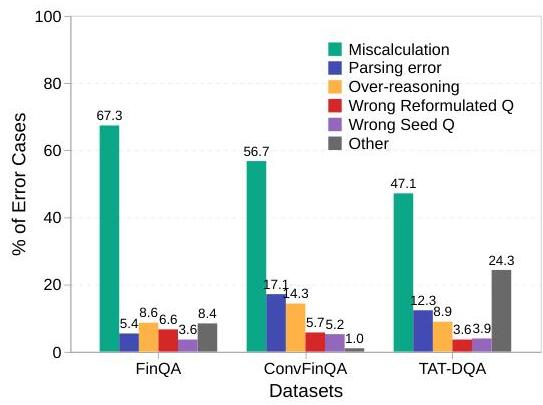
\includegraphics[width=0.8\linewidth]{figures/part2_img-1.jpeg}
    \caption{Results of the manual error analysis. Percentage of each error category per subset.}
\end{figure}

\section*{6 Conclusion}
In this paper, we introduced our newly created benchmark, $\mathbf{T}^2$-RAGBench, which contains 23,088 question-answer-context triples. It includes questions derived from over 7,318 documents and is designed to evaluate RAG methods for numerical reasoning over text-table data in the unknown context setting. While other datasets are defined in an \textit{Oracle Context}, our benchmark uses context-independent question making it possible to evaluate RAG methods. We demonstrate that our benchmark meets its intended goals through quantitative analysis and human validation. We test multiple RAG methods on the benchmark and find that \textit{Hybrid BM25}, which combines dense and sparse retrieval, performs best. Additionally, we conducted ablation studies showing that current SOTA embedding models achieve low R@5 and MRR@5 scores on text-and table contexts. With $\mathbf{T}^2$-RAGBench, we aim to facilitate the development of more RAG methods suitable for text-and-table documents, supporting the creation of real-world systems that can automatically analyze complex documents.
\section*{Limitations}
This section outlines the key limitations related to the methodology and dataset that may affect the validity and generalizability of the presented results.

\subsection*{Lack of Human Verification and Authenticity}
The questions used in the benchmark were generated synthetically, which can lead to distortions, as models do not inevitably generate the type of questions that real-world users would ask. Therefore, transferability to real systems may be affected. Although humans annotated the original question-answer pairs, there is no definitive guarantee that the generated questions will be formulated in a way that allows other models to answer them equivalently.

Another point is that a comprehensive verification process was only partly conducted on the benchmark questions. While we verified 100 samples per subset with four annotators in the benchmark, that the benchmark fulfills the requirements to be an evaluation dataset for our proposed task. Nevertheless, they can still be some questions that are not suitable to find the right context.

\subsection*{Domain-Specific Application}
The presented work aims to present a benchmark that can test text-table datasets from different document types with different knowledge. Nevertheless, the dataset consists only of financial documents that have the same standardized structure, consistent terminology, and domain-specific content. As a result, the model’s performance is tailored to this domain and can only be partly assumed to generalize to other types of document layouts or content types, such as medical reports, scientific publications, or administrative forms, where table-text relationships can vary significantly. Still, given the wide-ranging application of financial reporting standards, our work contributes to this specific domain.

\subsection*{Use of Quantized Models}
Due to limited resources, all evaluations were conducted using quantized versions of the models, which enabled faster inference times and the execution of large open-source models. While quantization offers clear advantages in terms of computational efficiency, it often comes at the cost of reduced numerical precision and model accuracy. Therefore, the performance may be lower than that of full-precision SOTA models. However, since the focus of this paper is on comparing suitable RAG methods, we consider this negligible.

\section*{Ethical Considerations}
This work introduces a benchmark dataset constructed from publicly available financial documents. All data used originates from previously published datasets (FinQA, ConvFinQA, TAT-DQA), which are either publicly accessible or sourced from publicly available company reports. No private, confidential, or personally identifiable information is included. The reformulated questions were synthetically generated using LLMs and subsequently validated by experts to ensure quality and context-independence. Human evaluation was conducted with informed consent and anonymized input. We acknowledge that while synthetic reformulation enhances benchmarking utility, it may not fully capture the natural distribution of user queries.

\section*{Acknowledgement}
This work is supported by the Genial4KMU project, Universität Hamburg, funded by BMBF (grant no. 16IS24044B).

\section*{References}
\begin{itemize}
    \item Akari Asai, Zeqiu Wu, Yizhong Wang, Avirup Sil, and Hannaneh Hajishirzi. 2024. Self-RAG: Learning to Retrieve, Generate, and Critique through Self-Reflection. In \textit{The Twelfth International Conference on Learning Representations}, Vienna, Austria. ICLR.
    \item Dipali Baviskar, Swati Ahirrao, Vidyasagar Potdar, and Ketan V. Kotecha. 2021. Efficient Automated Processing of the Unstructured Documents Using Artificial Intelligence: A Systematic Literature Review and Future Directions. \textit{IEEE Access}, 9:72894--72936.
    \item Jian Chen, Peilin Zhou, Yining Hua, Loh Xin, Kehui Chen, Ziyuan Li, Bing Zhu, and Junwei Liang. 2024. FinTextQA: A Dataset for Long-form Financial Question Answering. In \textit{Proceedings of the 62nd Annual Meeting of the Association for Computational Linguistics (Volume 1: Long Papers)}, pages 6025--6047, Bangkok, Thailand. Association for Computational Linguistics.
    \item Wenhu Chen, Hanwen Zha, Zhiyu Chen, Wenhan Xiong, Hong Wang, and William Yang Wang. 2020. HybridQA: A Dataset of Multi-Hop Question Answering over Tabular and Textual Data. In \textit{Findings of the Association for Computational Linguistics}, volume EMNLP 2020 of \textit{Findings of ACL}, pages 1026--1036, Online Event. Association for Computational Linguistics.
    \item Zhiyu Chen, Wenhu Chen, Charese Smiley, Sameena Shah, Iana Borova, Dylan Langdon, Reema Moussa, Matt Beane, Ting-Hao Huang, Bryan Routledge, and William Yang Wang. 2021. FinQA: A Dataset of Numerical Reasoning over Financial Data. In \textit{Proceedings of the 2021 Conference on Empirical Methods in Natural Language Processing}, pages 3697--3711, Online and Punta Cana, Dominican Republic. Association for Computational Linguistics.
    \item Zhiyu Chen, Shiyang Li, Charese Smiley, Zhiqiang Ma, Sameena Shah, and William Yang Wang. 2022. ConvFinQA: Exploring the Chain of Numerical Reasoning in Conversational Finance Question Answering. In \textit{Proceedings of the 2022 Conference on Empirical Methods in Natural Language Processing, EMNLP 2022}, pages 6279--6292, Abu Dhabi, United Arab Emirates. Association for Computational Linguistics.
    \item Chanyeol Choi, Jihoon Kwon, Jaeseon Ha, Hojun Choi, Chaewoon Kim, Yongjae Lee, Jy-yong Sohn, and Alejandro Lopez-Lira. 2025. FinDER: Financial Dataset For Question Answering And Evaluating Retrieval-Augmented Generation. In \textit{Proceedings Of The 6th ACM International Conference On AI In Finance}, pages 638--646, New York, NY, USA. Association for Computing Machinery.
    \item Chroma Team. 2025. Chroma: Open-Source Search And Retrieval Database For AI Applications. Https://github.com/chroma-core/chroma.
    \item Pradeep Dasigi, Kyle Lo, Iz Beltagy, Arman Cohan, Noah A. Smith, and Matt Gardner. 2021. A Dataset of Information-Seeking Questions and Answers Anchored in Research Papers. In \textit{Proceedings of the 2021 Conference of the North American Chapter of the Association for Computational Linguistics: Human Language Technologies}, pages 4599--4610, Virtual Event. Association for Computational Linguistics.
    \item Yongqi Fan, Hongli Sun, Kui Xue, Xiaofan Zhang, Shaoting Zhang, and Tong Ruan. 2025. MedOdyssey: A Medical Domain Benchmark for Long Context Evaluation Up to 200K Tokens. In \textit{Findings of the Association for Computational Linguistics: NAACL 2025}, pages 32--56, Albuquerque, New Mexico, USA. Association for Computational Linguistics.
    \item Luyu Gao, Zhuyun Dai, Tongfei Chen, Zhen Fan, Benjamin Van Durme, and Jamie Callan. 2021. Complement Lexical Retrieval Model With Semantic Residual Embeddings. In \textit{European Conference on Information Retrieval}, pages 146--160, Virtual Event. Springer.
    \item Luyu Gao, Xueguang Ma, Jimmy Lin, and Jamie Callan. 2023a. Precise Zero-Shot Dense Retrieval without Relevance Labels. In \textit{Proceedings of the 61st Annual Meeting of the Association for Computational Linguistics (Volume 1: Long Papers)}, pages 1762--1777, Toronto, Canada. Association for Computational Linguistics.
    \item Yunfan Gao, Yun Xiong, Xinyu Gao, Kangxiang Jia, Jinliu Pan, Yuxi Bi, Yi Dai, Jiawei Sun, Haofen Wang, and Haofen Wang. 2023b. Retrieval-Augmented Generation for Large Language Models: A Survey. \textit{Preprint}, arXiv:2312.10997.
    \item Michael Glass, Gaetano Rossiello, Md Faisal Mahbub Chowdhury, Ankita Naik, Pengshan Cai, and Alfio Gliozzo. 2022. Re2G: Retrieve, rerank, generate. In \textit{Proceedings of the 2022 Conference of the North American Chapter of the Association for Computational Linguistics: Human Language Technologies}, pages 2701--2715, Seattle, United States. Association for Computational Linguistics.
    \item Aaron Grattafori, Abhimanyu Dubey, Abhinav Jauhri, Abhinav Pandey, Abhishek Kadian, Ahmad Al-Dahle, Aiesha Letman, Akhil Mathur, Alan Schelten, Alex Vaughan, and 1 others. 2024. The Llama 3 Herd of Models. \textit{Preprint}, arXiv:2407.21783.
    \item Yulong Hui, YAO LU, and Huanchen Zhang. 2024. UDA: A Benchmark Suite for Retrieval Augmented Generation in Real-World Document Analysis. In \textit{Advances in Neural Information Processing Systems}, volume 37, pages 67200--67217, Vancouver, BC, Canada. Curran Associates, Inc.
    \item Zhengbao Jiang, Frank F. Xu, Luyu Gao, Zhiqing Sun, Qian Liu, Jane Dwivedi-Yu, Yiming Yang, Jamie Callan, and Graham Neubig. 2023. Active Retrieval Augmented Generation. In \textit{Proceedings of the 2023 Conference on Empirical Methods in Natural Language Processing}, pages 7969--7992, Singapore. Association for Computational Linguistics.
    \item Renren Jin, Jiangcun Du, Wuwei Huang, Wei Liu, Jian Luan, Bin Wang, and Deyi Xiong. 2024. A Comprehensive Evaluation of Quantization Strategies for Large Language Models. In \textit{Findings of the Association for Computational Linguistics: ACL 2024}, pages 12186--12215, Bangkok, Thailand. Association for Computational Linguistics.
    \item Mandar Joshi, Eunsol Choi, Daniel S. Weld, and Luke Zettlemoyer. 2017. TriviaQA: A Large Scale Distantly Supervised Challenge Dataset for Reading Comprehension. In \textit{Proceedings of the 55th Annual Meeting of the Association for Computational Linguistics}, pages 1601--1611, Vancouver, Canada. Association for Computational Linguistics.
    \item Pankaj Joshi, Aditya Gupta, Pankaj Kumar, and Manas Sisodia. 2024. Robust Multi Model RAG Pipeline For Documents Containing Text, Table \& Images. In \textit{2024 3rd International Conference on Applied Artificial Intelligence and Computing (ICAAIC)}, pages 993--999, Salem, India. IEEE.
\end{itemize}

\end{document}
